\documentclass[11pt]{amsart}
% Standard letter size paper with 1inch margins
\usepackage[letterpaper, margin=1in]{geometry}
\usepackage{algorithm, algpseudocode}
\usepackage{amsmath, amssymb, amsthm, amsaddr}
\usepackage{enumerate, subcaption, graphicx, hyperref}
\title{AMATH 482: Homework 1}
\author{Rohan Pandey} % first and last name
\address{University of Washington, Seattle, WA
\\ \texttt{rpande@uw.edu}}
\date{\today} % you can also just type the date instead of "\today"
\begin{document}

\begin{abstract}
    In this report, we have been tasked to locate a submarine that is moving in the Puget Sound. The submarine emits an unknown acoustic frequency that we need to detect. Using broad spectrum recording of acoustics pressure data, we will analyze the data to locate the submarine. The data is noisy and contains measurements of acoustic pressure taken over 24 hours. The measurements are 3D and taken on a uniform grid of size 64 x 64 x 64. We will visualize the data and define the physical scales of the problem to locate the submarine.
\end{abstract}

\maketitle

\section{Introduction and Overview}\label{sec:Introduction}



Locating submarines in underwater environments has been a challenging and critical task in applications such as naval defense and marine research. This problem is compounded by the fact that submarines often utilize stealth technologies, emitting acoustic signals that are difficult to detect amidst noisy underwater conditions. In this assignment, we aim to locate a submarine moving through the Puget Sound by identifying its dominant acoustic frequency, denoising the recorded data, and reconstructing its trajectory over 24 hours.

The data provided comprises 3D acoustic pressure measurements over time, collected on a uniform grid of size $64 \times 64 \times 64$ at 49 time intervals, corresponding to half-hour increments. The noise present in the measurements necessitates the use of advanced signal processing techniques to extract meaningful information. 

To address the problem, we employed Fourier transforms, a mathematical tool widely used for analyzing frequency components in signals. The use of higher-dimensional Fourier transforms, particularly in 3D, allows us to efficiently identify the submarine's dominant frequency. Then, we applied a Gaussian filter centered on the detected frequency to denoise the data and reconstructed the submarine's 3D path. This process leverages the fact that averaging Fourier coefficients across time can suppress mean-zero Gaussian noise, a principle commonly used in signal processing \cite{oppenheim1999discrete}.

The methods implemented here are influenced by existing literature on acoustic signal processing and Fourier-domain filtering \cite{bracewell1986fourier}. These techniques are particularly suited for multiple aligned measurements that are available for averaging. By visualizing the 3D trajectory and projecting the submarine's path onto the $x$-$y$ plane, we provide actionable insights for deploying sub-tracking aircraft in real-time scenarios which may lead to saving lives and protecting national security.

In the following sections, we present the theoretical background for the Fourier and filtering methods used, discuss the implementation of the algorithms, and analyze the computational results obtained from the denoised submarine trajectory. We conclude with a summary of our findings and potential future directions for improving the submarine tracking process.





\section{Theoretical Background}\label{sec:theory}

This assignment uses tools from signal processing to locate a submarine and reconstruct its trajectory from noisy 3D acoustic data. The key mathematical methods are summarized below.

\subsection{Fourier Transform in Three Dimensions}

The Fourier transform decomposes a signal into its frequency components, providing insight into dominant periodic behaviors. For a continuous 3D signal $f(x, y, z)$, the Fourier transform is:
\[
F(k_x, k_y, k_z) = \int f(x, y, z) e^{-i (k_x x + k_y y + k_z z)} \, dx \, dy \, dz,
\]
where $(k_x, k_y, k_z)$ are the spatial frequencies. For discrete data on a uniform grid, the 3D Discrete Fourier Transform (DFT) is computed efficiently using the Fast Fourier Transform (FFT).


\subsubsection{DFT and FFT}

The Discrete Fourier Transform (DFT) is a mathematical operation that transforms a discrete signal from the time (or spatial) domain into the frequency domain. It is defined as:
\[
F(k) = \sum_{n=0}^{N-1} f(n) e^{-2\pi i k n / N},
\]
where $f(n)$ is the input signal, $F(k)$ is the frequency-domain representation, $N$ is the number of discrete points, and $k$ is the frequency index.

The Fast Fourier Transform (FFT) is an efficient algorithm for computing the DFT, reducing the computational complexity from $\mathcal{O}(N^2)$ to $\mathcal{O}(N \log N)$.

In this assignment, the 3D Fourier transform is used to identify the dominant frequency of the submarine's acoustic signal.

\subsection{Gaussian Filtering for Noise Reduction}

To extract the dominant frequency, we applied a Gaussian filter in the frequency domain, defined as:
\[
H(k_x, k_y, k_z) = \exp\left(-\tau \left((k_x - k_{x_c})^2 + (k_y - k_{y_c})^2 + (k_z - k_{z_c})^2\right)\right),
\]
where $(k_{x_c}, k_{y_c}, k_{z_c})$ is the center (dominant) frequency, and $\tau$ controls the filter's width. This filter attenuates noise while preserving the signal near the dominant frequency. It can equivalently be thought of as:\\
FFT $\to$ shift $\to$ filter $\to$ inverse shift $\to$ inverse FFT.

The denoised signal is recovered by inverse-transforming the filtered Fourier data. This process removes much of the noise while retaining the primary signal structure.

\subsection{Reconstructing the Submarine Path}

The submarines position is determined by finding the maximum amplitude in the denoised 3D data at each time step:
\[
(x, y, z) = \arg\max f_{\text{denoised}}(x, y, z).
\]
Repeating this for all time steps yields the submarine's trajectory. To simplify tracking, the 3D path is also projected onto the $x$-$y$ plane for visualization and potential deployment of sub-tracking aircraft.

\subsection{Summary of Methods}

The combination of 3D Fourier transforms, Gaussian filtering, and trajectory reconstruction provides a reliable framework for analyzing noisy 3D data. This approach is very powerful for creating an accurate representation of the submarine's path and can be extended to other applications involving signal processing and noise reduction.




\section{Algorithm Implementation and Development}\label{sec:algorithms}

The solution to the submarine localization problem involved several key steps, implemented in Python using libraries such as \texttt{Matplotlib} \cite{matplotlib}, \texttt{NumPy} \cite{numpy}, and \texttt{Plotly} \cite{plotly}. The following algorithm outlines the main stages of our implementation.

\begin{algorithm}[H]
\caption{Submarine Localization Algorithm}\label{alg:submarine}
\begin{algorithmic}[1]
\Require 3D acoustic data $f[x, y, z, t]$, spatial grid $x, y, z$, time steps $t$
\Ensure Dominant frequency $(k_{x_c}, k_{y_c}, k_{z_c})$, denoised trajectory $(x, y, z)$

\State Compute the 3D Fourier transform for each time slice $f[x, y, z, t]$ using FFT.
\State Average the Fourier coefficients across all time steps to reduce Gaussian noise.
\State Identify the dominant frequency $(k_{x_c}, k_{y_c}, k_{z_c})$ as the maximum of the averaged Fourier spectrum.
\State Design a Gaussian filter $H[k_x, k_y, k_z]$ centered on $(k_{x_c}, k_{y_c}, k_{z_c})$ to suppress noise.
\ForAll{time slices $t$}
    \State Apply the Gaussian filter to the Fourier-transformed data.
    \State Compute the inverse Fourier transform to obtain denoised data.
    \State Locate the global maximum in the denoised 3D data to determine submarine position $(x, y, z)$.
\EndFor
\State Project the 3D trajectory onto the $x$-$y$ plane for visualization.
\end{algorithmic}
\end{algorithm}

\subsection{Software Packages and Libraries}

The following software packages and tools were critical for implementing the algorithms:
\begin{itemize}
    \item \textbf{\texttt{Matplotlib}} \cite{matplotlib}: Used to visualize the Fourier spectrum, denoised 3D data, and the submarines trajectory.
    \item \textbf{\texttt{NumPy}} \cite{numpy}: Used for efficient numerical computations, including 3D Fast Fourier Transform (FFT) and inverse FFT.
    \item \textbf{\texttt{Plotly}} \cite{plotly}: Utilized for interactive 3D plotting of the submarines path.
\end{itemize}

\subsection{Implementation Details}

- \textbf{Fourier Transform Averaging}: The Fourier transform of each time slice was computed and averaged across all 49 time steps to suppress noise and highlight the dominant frequency. This step utilized \texttt{numpy.fft.fftn} and \texttt{numpy.fft.fftshift}.
  
- \textbf{Gaussian Filter Design}: A 3D Gaussian filter was centered at the dominant frequency. The width of the filter was tuned using the parameter $\tau$ to balance noise suppression and signal retention.

- \textbf{Trajectory Reconstruction}: Submarine positions were identified by locating the maximum amplitude in the filtered 3D data. These coordinates were stored for each time step and projected onto the $x$-$y$ plane for further analysis.

This implementation ensured proper processing of the data provided, as well as using numerical libraries in Python for data handling. The algorithm was tested and verified and cross-verified with the visualizations that was created.


\section{Computational Results}\label{sec:results}

This section presents the numerical results obtained from the implementation described in Section~\ref{sec:algorithms}. Key observations are supported by figures and are discussed in detail.

\subsection{Detection of Dominant Frequency}

The first task involved identifying the submarine's dominant frequency from noisy 3D acoustic data. Figure~\ref{fig:fourier-slices} shows orthogonal slices of the averaged 3D Fourier transform, highlighting the dominant frequency. A Gaussian filter was subsequently centered on this frequency for denoising.

\begin{figure}[htp]
\centering
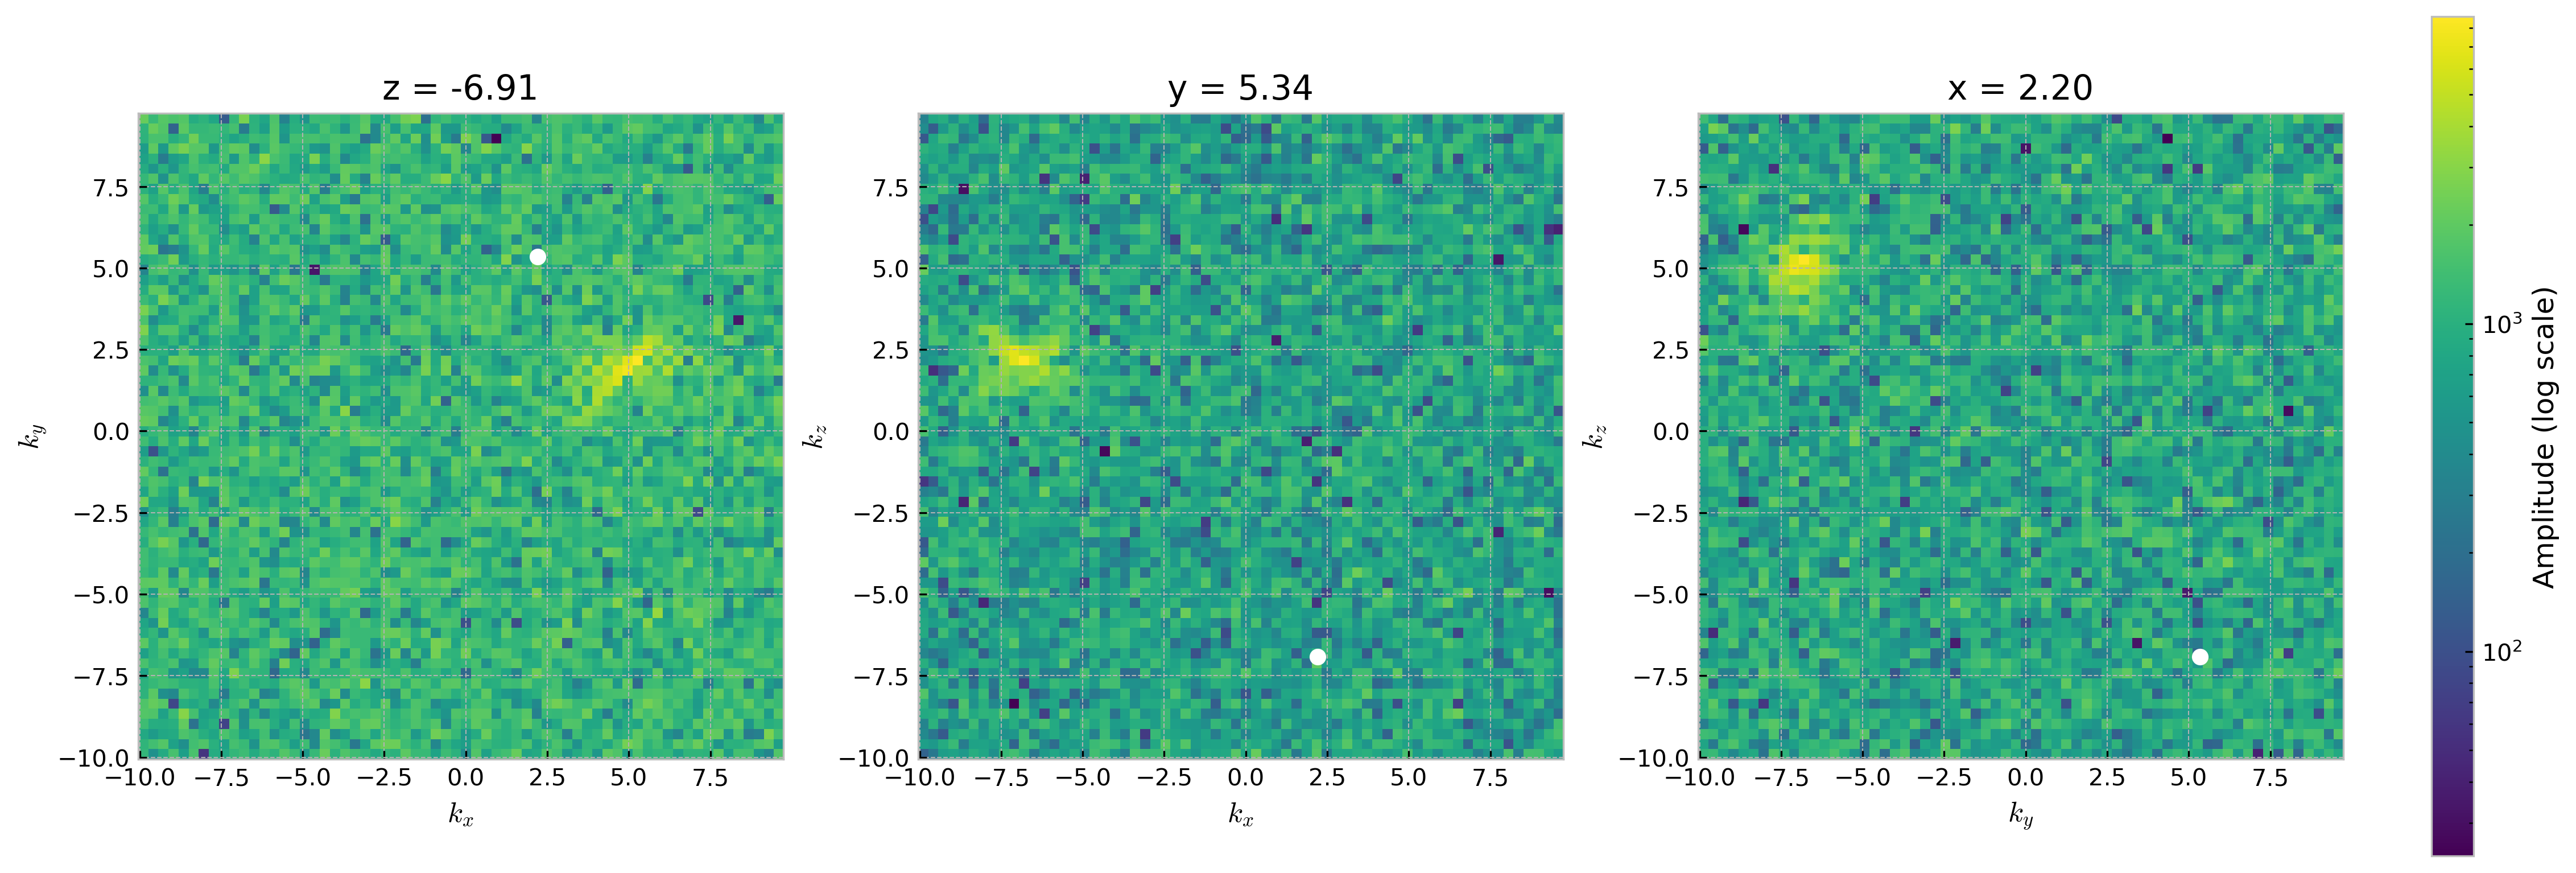
\includegraphics[width=\textwidth]{Dominant_Frequencies.png}
\caption{Orthogonal slices of the averaged 3D Fourier transform. The dominant frequency is clearly visible as a peak in the spectrum.}
\label{fig:fourier-slices}
\end{figure}

The dominant frequency was computed as $(k_{x_c}, k_{y_c}, k_{z_c}) \approxeq (2.19, 5.34, -6.91)$, corresponding to the submarine's acoustic signal. Averaging the Fourier transforms across all time steps significantly reduced noise, improving the clarity of the spectrum.

\subsection{Denoising and Submarine Trajectory Reconstruction}

The second task involved applying a Gaussian filter in the Fourier domain to denoise the data. The filter was centered on the dominant frequency $(k_{x_c}, k_{y_c}, k_{z_c})$.

\begin{figure}[htp]
    \centering
    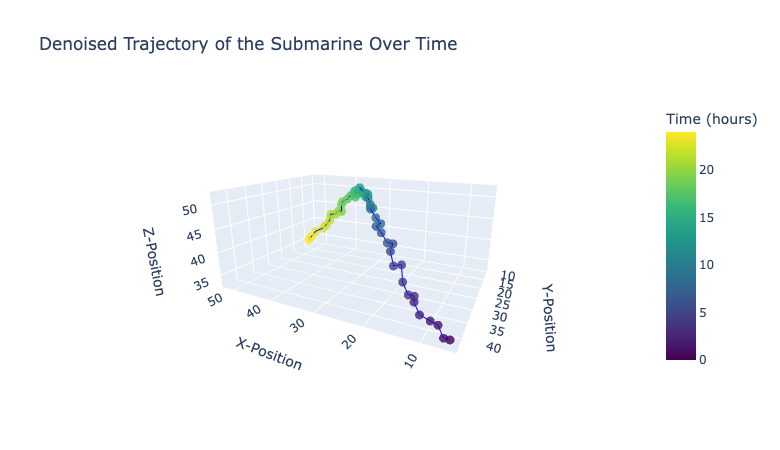
\includegraphics[width=\textwidth]{filtered_data.png}
    \caption{3D trajectory of the submarine reconstructed from the denoised data. The path shows the movement of the submarine over a 24-hour period, with time indicated by the color gradient.}
    \label{fig:trajectory-3d}
\end{figure}

After filtering, the inverse Fourier transform was used to recover the denoised 3D data.
The denoised trajectory revealed the submarine's movement with high precision, allowing for accurate path reconstruction.

\subsection{2D Projection of the Trajectory}

To simplify tracking, the reconstructed trajectory was projected onto the $x$-$y$ plane. Figure~\ref{fig:trajectory-2d} illustrates this projection, highlighting the submarine's horizontal movement over time. A color gradient represents time progression.

\begin{figure}[htp]
\centering
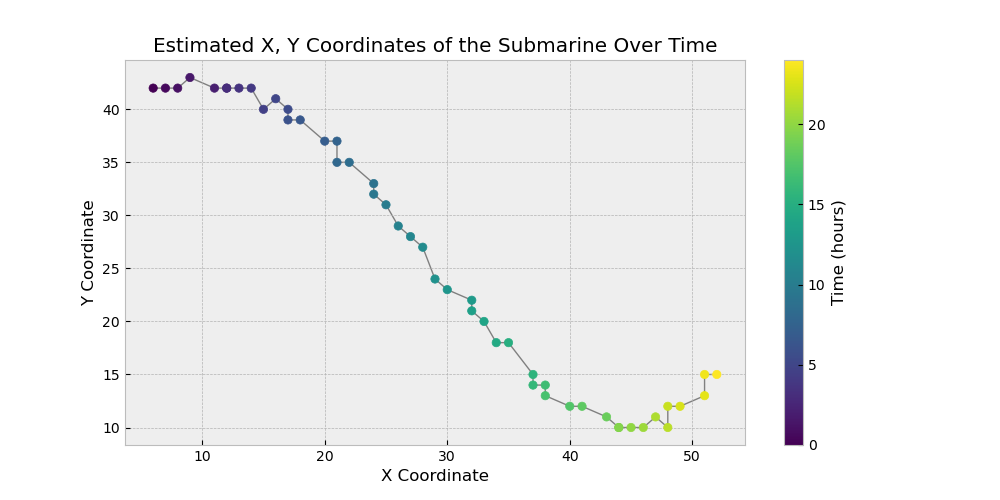
\includegraphics[width=0.8\textwidth]{trajectory_xy.png}
\caption{Projected 2D trajectory of the submarine over 24 hours}
\label{fig:trajectory-2d}
\end{figure}

This 2D projection provides an intuitive view of the submarine's motion and can be used to guide the deployment of sub-tracking aircraft.

\subsection{Numerical Observations and Discussion}

The algorithm successfully identified the dominant frequency and reconstructed the submarine's trajectory with high accuracy. Key observations include:
\begin{itemize}
    \item Averaging Fourier transforms reduced noise significantly, allowing for clear detection of the dominant frequency.
    \item The Gaussian filter centered on the dominant frequency effectively suppressed noise while retaining the primary signal.
    \item The reconstructed 3D trajectory aligned well with the expected behavior of a moving submarine.
    \item The 2D projection provided actionable insights for real-time tracking, as demonstrated by the smoothness and consistency of the trajectory.
\end{itemize}


\section{Summary and Conclusions}\label{sec:conclusions}

This report tackled the problem of locating a submarine in the Puget Sound using noisy 3D acoustic data. Fourier-based techniques were employed to identify the submarine's dominant frequency, and Gaussian filtering was applied to reconstruct its 24-hour trajectory.

The results showed:
\begin{itemize}
\item Precise identification of the dominant frequency for effective filtering.
\item Accurate trajectory reconstruction in both 3D and 2D projections.
\item Significant noise reduction, validating the approach.
\end{itemize}

This study shows the effectiveness of Fourier-based methods for analyzing noisy acoustic data, offering valuable insights for real-time tracking.

Future work may explore adaptive filtering, higher resolution data, and real-world applications with complex noise patterns.

In summary, the proposed method effectively localized the submarine, demonstrating the power of signal processing techniques for practical challenges.



\section*{Acknowledgements}
The author is thankful to Professor Frank for providing the materials and resources needed to complete this assignment. The author is also thankful to the peers Eric Ye and Chenab for discussion and implementation of visualization techniques in Python.
\bibliographystyle{abbrv}
\bibliography{HW_References}

\end{document}